\documentclass{article} % \documentclass{} is the first command in any LaTeX code.  It is used to define what kind of document you are creating such as an article or a book, and begins the document preamble

\usepackage{amsmath} % \usepackage is a command that allows you to add functionality to your LaTeX code
\usepackage{graphicx}
\graphicspath{ {./images/} }
\title{The Discrete Fourier Transform: Properties and Applications} % Sets article title
\author{Hunter Mills} % Sets authors name
\date{\today} % Sets date for date compiled

% The preamble ends with the command \begin{document}
\begin{document} % All begin commands must be paired with an end command somewhere
    \maketitle % creates title using information in preamble (title, author, date)
    These notes will only cover sections 7.1 through 7.4 in this chapter.\\
    
    Since the Discrete Time Fourier Transform (DTFT) produces a continuous function of frequency, it is not computationally convenient to use as a representation of $x[n]$. This chapter covers the representation of $x[n]$ by samples of its spectrum $X(\omega)$. This leads to the Discrete Fourier Transform (DFT) which is a powerful tool for preforming frequency analysis of signals.
    
    \section{Frequency Domain Sampling: The DFT} % creates a section
	This section covers the sampling of the DTFT of an aperiodic DT sequence and establish a relationship between the sampled DTFT and the DFT.
    
    \subsection{Frequency Domain Sampling and Reconstruction of DT Signals}
    Recall that aperiodic finite energy signals have continuous spectra and the DTFT can be calculated with
    \begin{equation}
	X(\omega) = \sum_n x[n]e^{-j\omega n}
	\end{equation}
	$X(\omega)$ is then sampled periodically in frequency at a spacing of $\delta \omega$ radians between samples. Since $X(\omega)$ is periodic with period $2\pi$ only samples from $0:2\pi$ or $-\pi:\pi$ are taken. We take $N$ samples in the interval $0 \le \omega < 2\pi$ with spacing $\delta \omega = 2\pi /N$ as shown in the figure 1. If we evaluate the DTFT equation at $\omega = 2\pi k/N$ we get
	
	\begin{figure}[h]
	\centering
	\includegraphics[width=10cm]{dft_s}
	\caption{Sampling DTFT Specrum}
	\end{figure}
	
	\begin{equation}
	X(\frac{2\pi}{N}k) = \sum_n x(n)e^{-j2\pi kn/N}, \;\;\;\; k = 0:N-1
	\end{equation}
	This can then be broken into an infinite number of summations where each sum contains $N$ terms. This is derived to be
	\begin{equation}
	X(\frac{2\pi}{N}k) = \sum_{n=0}^{N-1} [ \sum_l x(n-lN)]e^{-j2\pi kn/N}, \;\;\;\; k = 0:N-1
	\end{equation}
	From the inner summation
	\begin{equation}
	x_p(n) = \sum_l x(n-lN)
	\end{equation}
	is periodic with fundamental period $N$. It can be expanded into Discrete Time Fourier Coefficients (since it is now periodic) where
	\begin{equation}
	x_k = \frac{1}{N}\sum_{n=0}^{N-1} x_p(n)e^{-j2\pi kn/N}, \;\;\;\; k = 0:N-1
	\end{equation}
	By looking at (3) and (4) we can see
	\begin{equation}
	c_k = \frac{1}{N} X(\frac{2\pi}{N}k), \;\;\;\; k = 0:N-1
	\end{equation}
	Therefore 
	\begin{equation}
	x_p(n) = \frac{1}{N}\sum_{k=0}^{N-1} X(\frac{2\pi}{N}k) e^{-j2\pi kn/N}, \;\;\;\; n = 0:N-1
	\end{equation}
	This provides a reconstruction of the periodic signal $x_p(n)$ from $X(\omega)$. Since $x_p(n)$ is the periodic extension of $x(n)$ we can recover $x(n)$ if there is no aliasing in the time domain (ie: $x(n)$ is time limited to less than N samples). When $x(n)$ is zero outside the interval $0 \le n \le L - 1$, $N \ge L$ and $x(n)$ can be recovered without aliasing. This is shown in figure 2. Thus the spectrum of an aperiodic DT signal with finite duration L can be exactly recovered from its samples at frequencies $\omega_k = 2\pi k/N$ if $N \ge L$. 
	
	\begin{figure}[h]
	\centering
	\includegraphics[width=10cm]{dft_alias}
	\caption{Time Domain Aliasing}
	\end{figure}
	
	\subsection{The DFT}
   In general the frequency samples shown in the previous subsection do not uniquely represent $x(n)$ if it is infinite. Instead the samples correspond to $x_p(n)$ which is the periodic extension of $x(n)$ when $x(n)$ is finite. The \textbf{DFT} of a DT finite signal $x(n)$ is defined as 
    \begin{equation}
	X(k) = X(\frac{2\pi k}{N}) = \sum_{n=0}^{N-1} x(n)e^{-j2\pi kn/N}, \;\;\;\; k = 0:N-1
	\end{equation}
	And the \textbf{IDFT} is defined as 
    \begin{equation}
	x(n) = \frac{1}{N}\sum_{k=0}^{N-1} X(k)e^{j2\pi kn/N}, \;\;\;\; n = 0:N-1
	\end{equation}
	
	\subsection{The DFT as a Linear Transform}
	The DFT and IDFT can be expressed as
	\begin{equation}
	X(k) = \sum_{n=0}^{N-1} x(n)W_N^{kn}, \;\;\;\; k = 0:N-1
	\end{equation}
    \begin{equation}
	x(n) = \frac{1}{N}\sum_{k=0}^{N-1} X(k)W_N^{-kn}, \;\;\;\; n = 0:N-1
	\end{equation}
	where
	\begin{equation}
	W_N = e^{-j2\pi /N}
	\end{equation}
	is the $N$ th root of unity. The computation of each point of the DFT can be done by $N$ complex multiplies and $(N-1)$ complex additions. Hence the $N$-point DFT can be computed in $N^2$ complex multiplies and $N(N-1)$ complex additions. Define $\textbf{x}_N$ as an $N$-point vector of the sequence $x(n)$, $\textbf{X}_N$ of frequency samples and an $N \times N$ matrix $\textbf{W}_N$. These vectors/matrices are shown in the next figure. 
  
	\begin{figure}[h]
	\centering
	\includegraphics[width=10cm]{roots_w}
	\caption{Vector Representation of DFT}
	\end{figure}
	
	Using these definitions the $N$-point DFT can be expressed in matrix form as\
	\begin{equation}
	\textbf{X}_N = \textbf{W}_N \textbf{x}_N
	\end{equation}
	The IDFT can be expressed as 
	\begin{equation}
	\textbf{x}_N = \frac{1}{N}\textbf{W}_N^* \textbf{X}_N
	\end{equation}
	where $\textbf{W}_N^*$ if the complex conjugate of the matrix $\textbf{W}_N$
	
	\subsection{Relationship of the DFT to other Transforms}
	Most of the equations were derived previously.\\
	\textbf{Relationship to the FS coefficients of a DT periodic sequence}\\
	This relationship uses $x_p(n)$ and $c_k$.
	\begin{equation}
	X(k) = Nc_k
	\end{equation}
	\textbf{Relationship to the FT of an DT aperiodic sequence}\\
	This was derived heavily in these notes, but the only case where the IDFT will produce $x(n)$ from $X(k)$ is when $x(l)$ is finite and $L \le N$.\\
	\textbf{Relationship to the z-transform}\\
	The z-transform is
	\begin{equation}
	X(z) = \sum_n x(n)x^{-z}
	\end{equation}
	with a region of convergence that includes the unit circle. When $X(z)$ is sampled at $z_k = e^{j2\pi k/N}$ we obtain
	\begin{equation}
	X(k) = X(z)|_{z=e^{j2\pi k/N}} = \sum_n x(n)e^{-j2\pi kn/N}, \;\;\;\; k = 0:N-1
	\end{equation}
	\textbf{Relationship to the FS coefficients of a CT signal}\\
	The CT signal with fundamental period $T_p = 1/F_0$ can be expressed as 
	\begin{equation}
	x_a(t) = \sum_k c_ke^{j2\pi ktF_0}
	\end{equation}
	If we sample this at $F_s = N/T_p = 1/T$ it produces
	\begin{equation}
	x(n) = x_a(nT) = \sum_{k=0}^{N-1} [ \sum_l c_{k-lN}]e^{j2\pi kn/N}
	\end{equation}
	Thus the FS coefficients are aliased (copied in time).\\
	
	\subsection{Take Away}
	The DFT $X(k)$ is a set of $N$ points sampled from $X(\omega)$ for the finite duration signal $x(n)$. The sampling occurs at the N equally spaced frequencies $\omega_k = 2\pi k/N, \;k=0:N-1$ and uniquely represents $x(n)$ in the frequency domain. 
	\section{Properties of the DFT}
	This section covers the important properties of the DFT, which resemble the properties of the other transforms covered so far. 
	\begin{equation}
	x(n) \leftrightarrow_N^{DFT} X(k)
	\end{equation}
	\subsection{Periodicity, Linearity and Symmetry Properties}
	\textbf{Periodicity:} Both $x(n)$ and $X(k)$ are periodic with N.\\
	\textbf{Linearity:} $a_1x_1(n) + a_2x_2(n)\\ \leftrightarrow_N^{DFT} a_1X_1(k) + a_2X_2(k)$
	\textbf{Circular Symmetries of a Sequence:} The $N$-point DFT of finite duration signal $x(n)$ of length $L \le N$ is equivalent to the $N$-point DFT of the periodic sequence $x_p(n)$ which is obtained by periodically extending x(n)
	\begin{equation}
	x_p(n) = \sum_l x(n-lN)
	\end{equation}
	\begin{equation}
	x_p'(n) = x_p(n-k) = \sum_l x(n-k-lN)
	\end{equation}
	\begin{equation}
	x'(n) =  \begin{cases}
      		x_p'(n), & \;\;\; 0 \le n \ne N-1 \\
      		0, & \text{otherwise}
    	\end{cases} 
	\end{equation}
	$x_p(n)$ is able to be shifted in time and that is called \textit{circular shift} and it is demonstrated in the following figure. In general the circular shift can be represented as the index mod N
	\begin{equation}
	x'(n) = x((n-k) mod N)
	\end{equation}

	\begin{figure}[h]
	\centering
	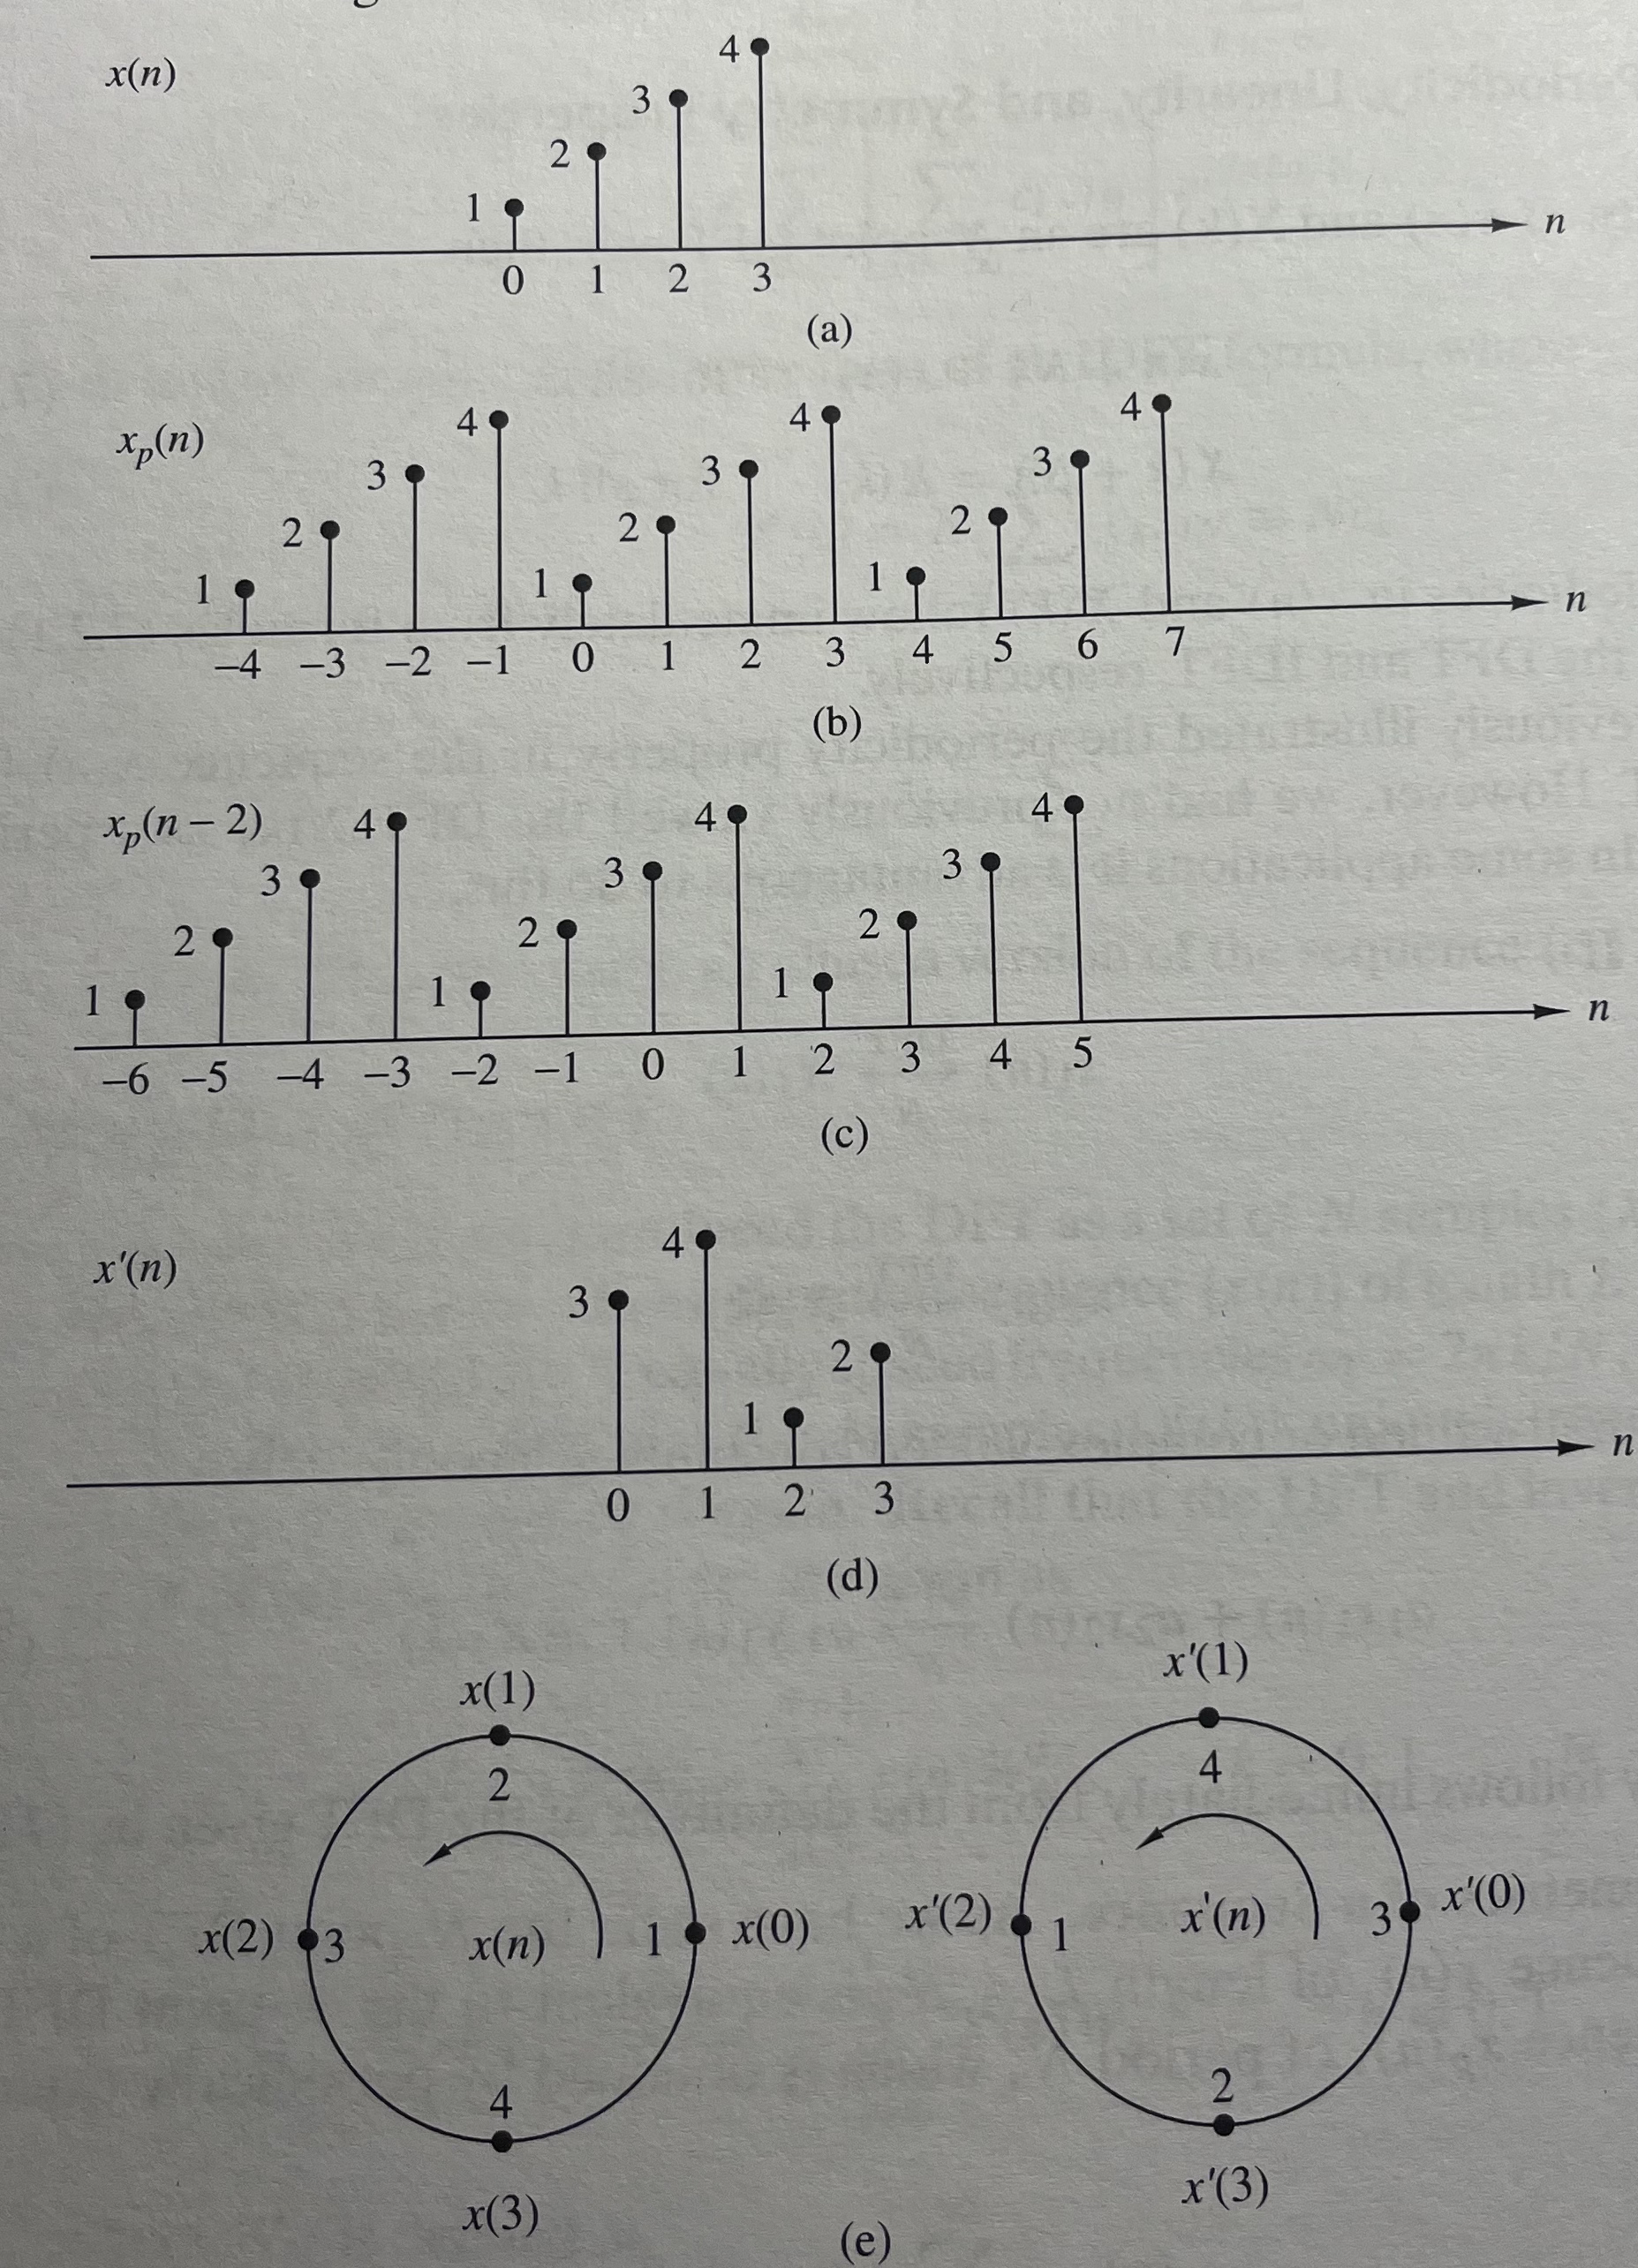
\includegraphics[width=10cm]{circ_shift}
	\caption{Circular Shifting a Signal}
	\end{figure}
	
	For example if $k = 2$ and $N = 4$, $x'(n) = x((n-2) mod 4$. A circular shift of an $N$-point sequence if equivalent to a linear shift of its periodic extension. 
	
	A $N$-point sequence is \textit{circularly even} if it is symmetric about point zero on a circle ($x(N-n) = x(n), \; 1 \le n \le N-1$). A $N$-point sequence is \textit{circularly odd} if it is antisymmetric about point zero on a circle ($x(N-n) = -x(n), \; 1 \le n \le N-1$). The time reversal of an $N$-point sequence is by reversing its samples about the point zero,
	\begin{equation}
	x((-n))_N = x(N-n) \;\;\;\; 0 \le n \le N-1
	\end{equation}
	\textbf{Symmetry Properties of the DFT:} These relationships are shown in the next figure. If $x(n)$ is real and even then $X(k)$ will be real and even. If $x(n)$ is real and odd then $X(k)$ will be imaginary and odd. If $x_I(n)$ if odd the $X_I(k) = 0$ and $X(k)$ is real. If $x_I(n)$ if even then $X_R(k) = 0$ and $X(k)$ is imaginary. 
	
	\begin{figure}[h]
	\centering
	\includegraphics[width=10cm]{symm_dft}
	\caption{Symmetry Properties of DFT}
	\end{figure}
	
	\subsection{Multiplication of Two DFTs and Circular Convolution}
	Say we have two finite signals of length $N$, $x_1(n)$ and $x_2(n)$. $x_3(n)$ is produced by multiplying the spectrum's of the first two signals. 
	\begin{equation}
	x_3(m) = \frac{1}{N} \sum_{k=0}^{N-1} X_1(k)X_2(k)e^{j2\pi km/N}
	\end{equation}
	The following is derived in the book but results in \textbf{circular convolution}.
	\begin{equation}
	x_3(m) = \sum_{n=0}^{N=1}x_1(n)x_2((n-m) mod N), \;\;\;\; m = 0:N-1
	\end{equation}
	The multiplication of two DFT's is equivalent to circular convolution in the time domain. Good example 472 and 475.
	
	\subsection{Additional DFT Properties}
	All of these properties have more details in the book but the following figure shows the properties. 
	
	\begin{figure}[h]
	\centering
	\includegraphics[width=10cm]{prop_dft}
	\caption{Properties of DFT}
	\end{figure}
	
	\section{Linear Filtering Methods Based on the DFT}
	In this section we will look at a computational procedure that serves as an alternate to time domain convolution. Additionally FFT's are more computationally efficient than time domain convolution. 
	\subsection{Use of the DFT in Linear Filtering}
	In the previous section it was shown that the multiplication of two spectrum's in the frequency domain is circular convolution in the time domain. But circular convolution isnt much help if we want to determine the output of a linear filter to a given input sequence. 
	We have a finite duration sequence $x(n)$ of length L which is input to a FIR filter of length M.
	\begin{equation}
	x(n) = 0 \;\;\;\; n < 0 \text{ and } n \ge L
	\end{equation}
	\begin{equation}
	h(n) = 0 \;\;\;\; n < 0 \text{ and } n \ge M
	\end{equation}
	The output of the FIR filter $y(n)$ is
	\begin{equation}
	y(n) = \sum_{k=0}^{M-1}h(k)x(n-k)
	\end{equation}
	\begin{equation}
	Y(\omega) = X(\omega)H(\omega)
	\end{equation}
	Since $h(n)$ and $x(n)$ are finite duration, their convolution is also finite and is $L + M -1$. To represent $y(n)$ uniquely in the frequency domain the DFT size N must satisfy $N \ge L + M -1$. To make circular convolution equivalent to linear convolution of $x(n)$ and $h(n)$, $x(n)$ and $h(n)$ need to be zero padded to a length of $N$. 
	\subsection{Filtering of Long Data Sequences}
	In practical applications $x(n)$ is often a very long sequence. Since linear filtering preformed via the DFT involves operations on a block of data a long input signal must be segmented. Since filtering is linear, successive blocks can be processed and the fitted back together. The two methods looked at in this section are \textit{overlap-save} and \textit{overlap-add} methods. We assume that the FIR filter has a duration M and $L >> M$. \\
	\textbf{Overlap-save Method}\\
	The size of the input data block is $N = L + M -1$ and the DFT's are of length $N$. Each data block had $M-1$ data points of the previous data block followed by $L$ new data points to form a sequence of length $N$. Then an DFT is calculated for each block and on the zero-padded impulse response. For the $m^{th}$ block the response is
	\begin{equation}
	\hat{Y}_m = H(k)X_m(k)
	\end{equation}
	Since the data length is of length $N$ the first $M-1$ samples must be discarded due to aliasing and the remaining $L$ samples are equivalent to the time domain linear convolution. 
	\begin{equation}
	\hat{y}_m(n) = y_m(n), \;\;\;\; n = M:N-1
	\end{equation}
	The discarded $M-1$ samples are then used to pad the next $L$ new samples. This method is shown in the next figure.
	
	\begin{figure}[h]
	\centering
	\includegraphics[width=7cm]{os}
	\caption{Overlap-save Algorithm}
	\end{figure}
	\textbf{Overlap-add method}\\
	This method is very similar except for padding the beginning of the signal with $M-1$ old samples, we pad the end of $L$ samples with $M-1$ zeros. We then add the signal blocks together overlapping by $M-1$ samples and is shown in figure 8.
	
	\begin{figure}[h]
	\centering
	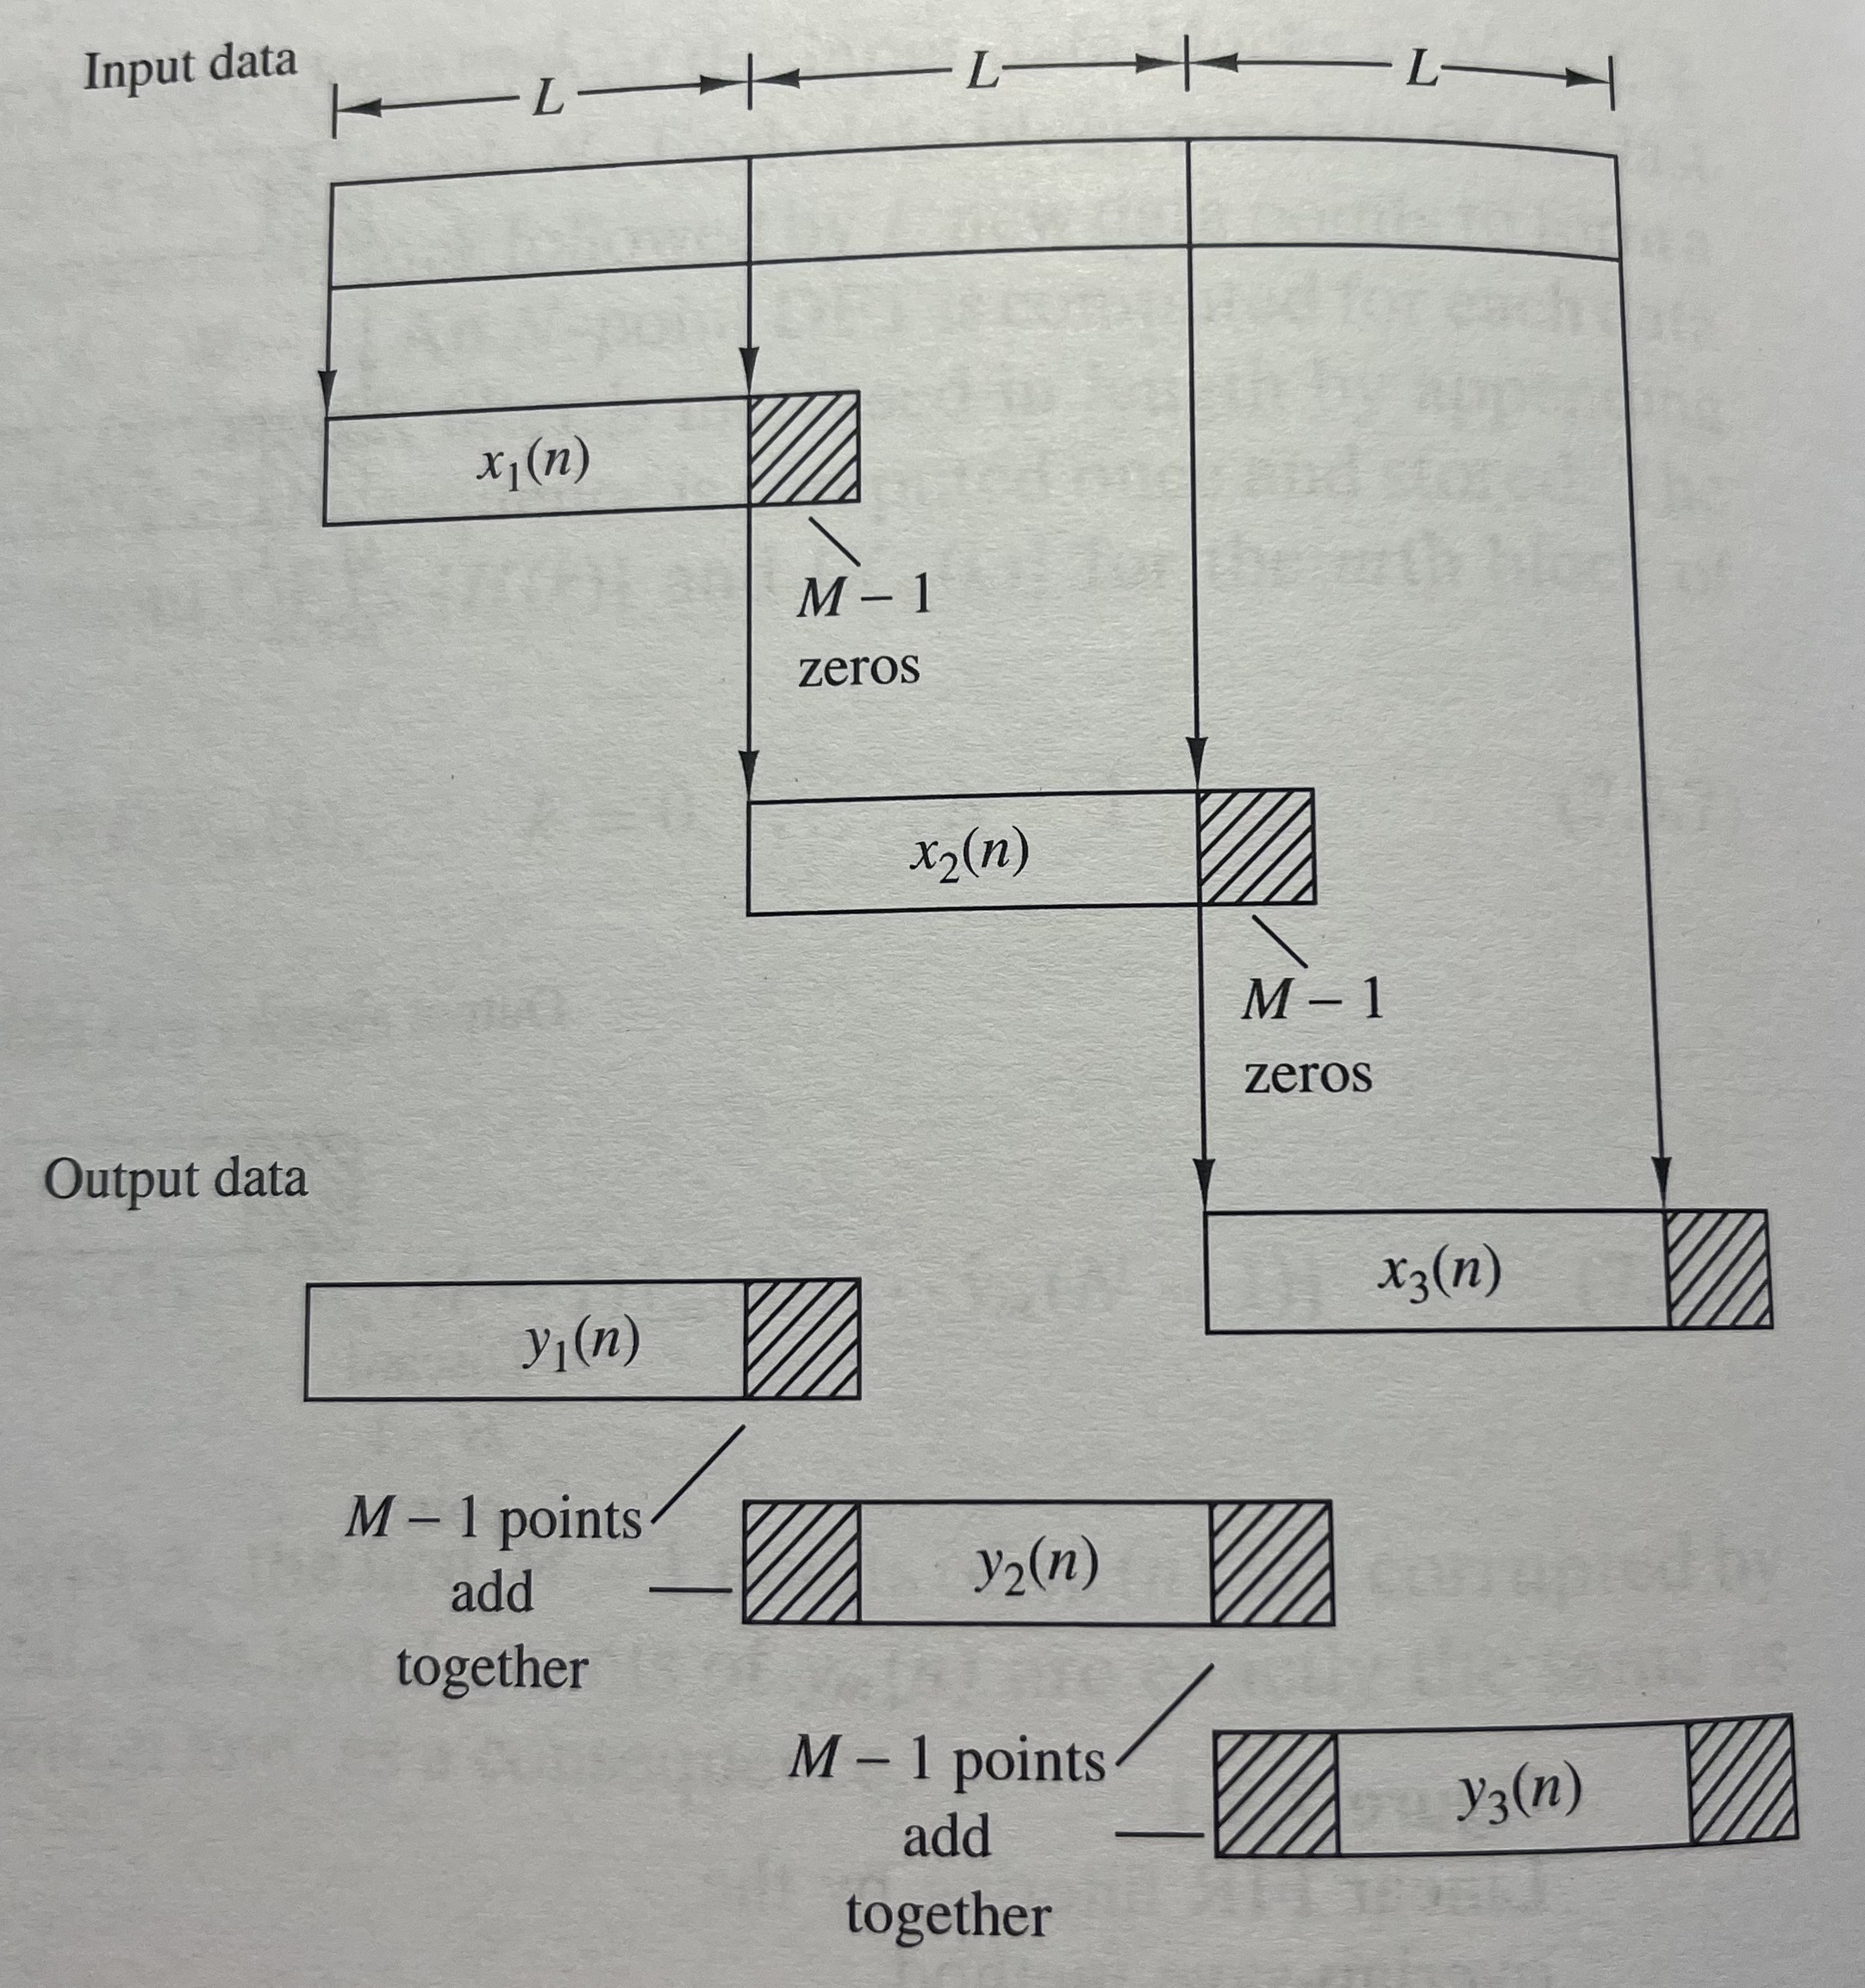
\includegraphics[width=7cm]{oa}
	\caption{Overlap-add Algorithm}
	\end{figure}
	
	\section{Frequency Analysis of Signals using the DFT}
	To take a DFT of a real world signal, first send through an antialiasing filter, sample at $F_s \ge 2B$ and limit the duration of the signal to $T_o = LT$ where $L$ is the number of samples and T is the sample interval.The finite signal observation limits the frequency resolution between two samples to $1/LT$. In order to time limit the signal we use windowing which makes the frequency from the signal leak into other frequency bins. For a general signal $x(n)$ windowed with $w(n)$ the frequency domain spectrum is 
	\begin{equation}
	\hat{X}(\omega) = \frac{1}{2\pi}\int_{-\pi}^{\pi} X(\theta)W(\omega - \theta)d\theta
	\end{equation}
	and the DFT of that signal is
	\begin{equation}
	\hat{X}(k) = \frac{1}{2\pi} \int_{-pi}^{\pi} X(\theta)W(\frac{2\pi k}{N} - \theta)d\theta, \;\;\;\; k=0:N-1
	\end{equation}
	
\end{document} % This is the end of the document